\documentclass{article}
\usepackage[utf8]{inputenc}
\usepackage{graphicx}
\usepackage[spanish]{babel}
\usepackage{amsmath}
\usepackage{vmargin}
\setpapersize{A4}
\setmargins{2.5cm}       % margen izquierdo
{1.5cm}                        % margen superior
{16.5cm}                      % anchura del texto
{23.42cm}                    % altura del texto
{10pt}                           % altura de los encabezados
{1cm}                           % espacio entre el texto y los encabezados
{0pt}                             % altura del pie de página
{2cm}                           % espacio entre el texto y el pie de página
\title{Número de estados de un cubo 2x2x2}
\author{Andoni Latorre Galarraga}
\date{}

\begin{document}

\maketitle

\begin{center}
    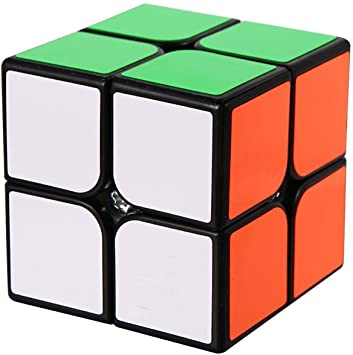
\includegraphics[scale=0.75]{figuras/61D7znf3r-L._AC_SY355_.jpg}
\end{center}
\pagebreak
\noindent Un estado de un cubo de rubik 2x2x2 es el resultado de hacer varios giros a partir del estado resuelto. La orientación en la que se sostenga el cubo no afecta realmente al estado por lo que contaremos las diferentes orientaciones del cubo como un mismo estado. Para calcular el número de estados es necesario ver que no todas las posiciones que nos podemos imaginar están conectadas al estado resuelto por medio de giros. Primero veremos a que estados se puede llegar por medio de giros y luego, conociendo las restricciones, calcularemos cuantos estados existen.\\\\
\noindent\textbf{Lema 1}\\
Si $C_n=\{1,2,\cdots,n\}$ y definimos $g_{(i,j)}$ como
$$
\begin{array}{cccc}
    g_{(i,j)}: & C_n & \longrightarrow & C_n\\
               & x   & \longmapsto     & \left\{ \begin{array}{cc}
                                                 x &  x\notin \{i,j\}\\
                                                 i &  x=j\\
                                                 j &  x=i
                                                 \end{array}\right.
\end{array}
$$
entonces cualquier aplicación biyectiva de $C_n$ en $C_n$ se puede escribir como composición de $g_{(i,j)}$.\\
\textit{Demostración:}\\
Sean $K=\{ x\in C_n : f(x)=x \}$ y $V=\{ x\in C_n : f(x)\ne x \}$ donde $f$ es la aplicación biyectiva. Evidentemente $C_n$ es la unión disjunta de $K$ y $V$. Visto esto, sólo queda demostrar que $f_{|V}$ se puede escribir como composición de $g_{(i,j)}$. sea $V=\{ v_1, v_2, \cdots, v_m \}$. Construimos tuplas de la siguiente forma:
$$
\begin{array}{ccc}
    v_1 \in L & T = (v_1, \underbrace{f(v_1)}_{v_{l_1}}, \underbrace{f(v_{l_1})}_{v_{l_2}}, \underbrace{f(v_{l_2})}_{v_{l_3}}, \cdots , \underbrace{f(v_{l_q})}_{v_1}) & L=\{v_1,v_{l_1},v_{l_2}, \cdots, v_{l_q} \} \\
    v_{l^\prime_0} \in V^\prime = V-L & T^\prime = (v_{l^\prime_0}, \underbrace{f(v_{l^\prime_0})}_{v_{l^\prime_1}}, \underbrace{f(v_{l^\prime_1})}_{v_{l^\prime_2}}, \underbrace{f(v_{l^\prime_2})}_{v_{l^\prime_3}}, \cdots , \underbrace{f(v_{l^\prime_{q^\prime}})}_{v_{l^\prime_0}}) & L^\prime=\{ v_{l^\prime_0}, v_{l^\prime_1} , \cdots , v_{l^\prime_{q^\prime}} \} \\
    v_{l^{\prime \prime}_0} \in V^{\prime \prime} = V^\prime - L^\prime & \vdots & \vdots \\
    \vdots & \vdots & \vdots \\
\end{array}
$$
El proceso termina cuando se llega a que el primer elemento de la tupla tiene que pertenecer a $\emptyset$. El tamaño de las tuplas y el número de tuplas siempre va a ser finito por ser $V$ finito. Por ser las tuplas disjuntas 2 a 2 se tiene que $f_{|L^{(a)}} \circ f_{|L^{(b)}} = f_{|L^{(b)}} \circ f_{|L^{(a)}}$. Entonces, $f=f_{|L} \circ f_{|L^\prime} \circ f_{|L^{\prime \prime}} \circ \cdots$ y sólo queda demostrar que $f_{|L^{(a)}}$ se puede escribir como composición de $g_{(i,j)}$. Sea $T^{(a)}=(t_1, t_2, \cdots, t_s, t_1)$ entonces, $f_{|L^{(a)}} = g_{(t_1,t_2)} \circ g_{(t_2, t_3)} \circ \cdots \circ g_{(t_{s-1}, t_s)}$ y queda probado el lema.\\\\
\textbf{Lema 2}\\
Existe una sucesión de giros que intercabia 2 esquinas adyacentes en un cubo 2x2x2.\\
\textit{Demostración:}\\
R U R' U' R' F R2 U' R' U' R U R' F' \dag\\\\
\textbf{Corolario 2.1}\\
Se pueden intercambiar 2 esquinas cualesquiera.\\
\textit{Demostración:}\\
Siempre podemos sujetar el cubo de manera que una de las esquinas quede en la mitad derecha y la otra enla mitad izquierda. Giramos el lado derecho hasta que sean adyacemtes las intercambiamos y deshacemos el giro inicial.\\\\
\noindent\textbf{Teorema 1}\\
Cualquier permutación de las 8 esquinas de un cubo 2x2x2 (sin tener en cuenta la orientación de estas) se puede conseguir con al menos una sucesión de giros.\\
\textit{Demostración:}\\
Si numeramos las esquinas del cubo la permutación pasa a ser una aplicación biyectiva de $C_8$ en $C_8$. Descomponemos esta aplicación en una composición de $g_{(i,j)}$ y obtenemos una lista de intercambios de 2 esquinas que tenemos que hacer para obtener la permutación. Como todos los intercambios de 2 esquinas son posibles, corolario 2.1, se tiene que todas las permutaciones son posibles.\\\\
\textbf{Teorema 2}\\
La orientación de una esquina depende de la orientación de las otras 7.\\
\textit{Demostración:}\\
Primero vamos a dar un valor numérico a la orientación de cada esquina. Todas las esquinas tienen o una pegatina amarilla o una blanca, pero no las 2 ya que el blanco y el amarillo están en caras opuestas en el estado resuelto. Para la mitad de arriba, si la esquina tiene la pegatina blanca/amarilla hacia arriba su orientación vale 0, si necesita un giro en el sentido contrario a las agujas del reloj para que la pegatina blanca/amarilla esté hacia arriba vale 1 y si necesita un giro en el sentido de las agujas del reloj vale 2. Para la cara de abajo, lo mismo pero con lo que necesita para que la pegatina blanca/amarilla esté hacia abajo.\\\\
Veamos que la suma de las orientaciones siempre es 0 módulo 3. En el estado resuelto todas las orientaciones valen 0. Ahora, vamos a ver que los giros conservan la propiedad.\\\\
Para los giros de las caras de arriba y abajo es evidente ya que estos no afectan a la orientación.\\\\
Para los giros laterales:
\begin{center}
    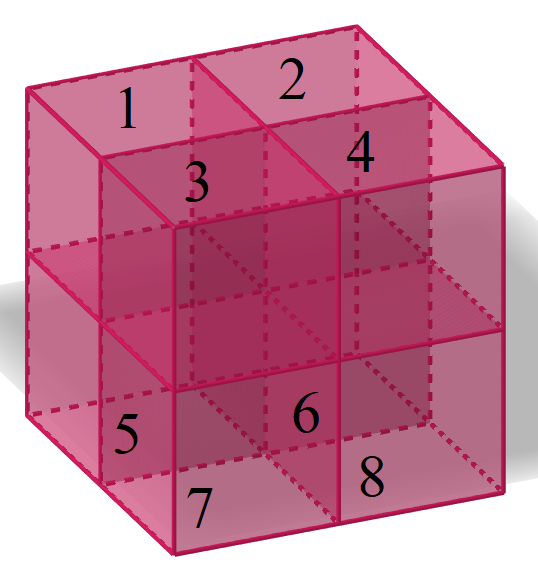
\includegraphics[scale=0.25]{figuras/cubo rosa.PNG}
\end{center}
Supongamos, sin pérdida de generalidad, que hacemos el giro $\overleftarrow{3\to4\to8\to7}$. Si llamamos $0(n)$ a la orientación de la esquina $n$.
$$
\begin{tabular}{|c|c|c|} \hline
    & \text{Antes del giro} & \text{Despues del giro} \\ \hline
    & o(1) & o(1) \\
    & o(2) & o(2) \\
    & o(3) & o(3)+1 \\
    & o(4) & o(4)+2 \\
    & o(5) & o(5) \\
    & o(6) & o(6) \\
    & o(7) & o(7)+2 \\
    & o(8) & o(8)+1 \\ \hline
    \text{Total módulo 3} & 0 & 0+6 \equiv 0 \\ \hline
\end{tabular}
$$
Se tiene que la propiedad se cumple siempre.\\\\
\underline{Nota:}\\
Conociendo la orientación de 6 esquinas no se puede saber la de las 2 restantes. Por ejemplo:\\
(R U R' U' R' F R2 U' R' U' R U R' F')\\
(R U R' U R U2 R2 U' R U' R' U2 R)\\
(R' U2 R U R' U R2 U2 R' U' R U' R') \dag\\\\
\textbf{Teorema 3}\\
El cubo 2x2x2 tiene 3.674.160 estados posibles.\\
\textit{Demostración:}\\
Primero calculamos el número de permutaciones de las esquinas, que es $P_8 = V_{8,8} = 8!$. Las posibles orientaciones de esas esquinas son $VR_{3,7}=3^7$. Como la orientación en la que sujetemos el cubo no importa, tenemos que dividir entre el número de orientaciones. 6 caras para elegir cual es la de arriba y 4 para elegir cual es la de la derecha. Se tiene:
$$
\frac{8! \cdot 3^7}{6 \cdot 4} = 3.674.160
$$
\dag https://www.iberorubik.com/tutoriales/2x2x2/notation/
\end{document}
